\documentclass[border=4pt]{standalone}
\usepackage{pgfplots}
\pgfplotsset{compat=newest}

\begin{document}
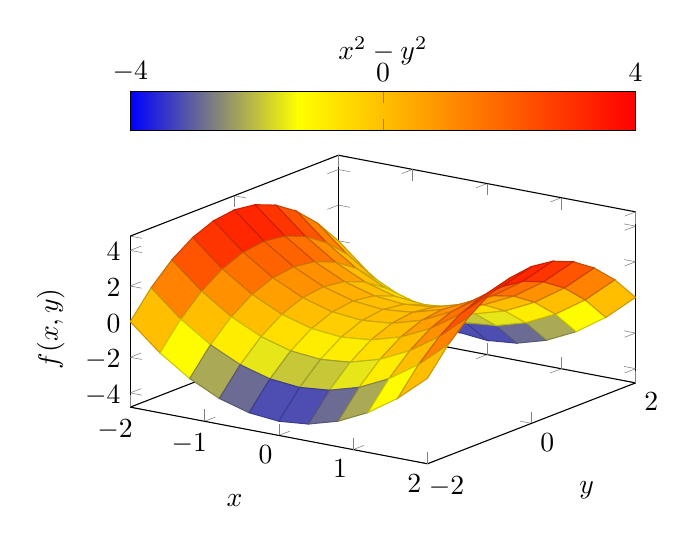
\begin{tikzpicture}
  \begin{axis}[
    width=8cm,
    height=5.5cm,
    view={35}{30},
    domain=-2:2,
    y domain=-2:2,
    samples=11,
    xlabel={$x$},
    ylabel={$y$},
    zlabel={$f(x,y)$},
    colorbar horizontal,
    colorbar style={
      at={(0.5,1.08)},
      anchor=south,
      xtick={-4,0,4},
      xticklabel pos=top,
      title={$x^2-y^2$}
    }
  ]
    \addplot3[surf] {x*x-y*y};
  \end{axis}
\end{tikzpicture}
\end{document}
